\begin{frame}[t]{Branch decomposition and MIM-width}
	\begin{itemize}[<+->]
		\item A \textbf{branch decomposition} $T$ of a graph $G = (V, E)$ is a binary rooted tree $T$, whose leaves are in one-to-one correspondence with $V$.
		\item The maximal-induced-matching width (MIM-width) of a vertex $t$ of $T$ is the size of a largest induced matching $M$ of $G[V\setminus V_t, V_t]$.
		\item $mimw(T) = \max\{MIM-width(t) : t \in V(T)\}$.
	\end{itemize}

	\uncover<4->{
	Example.

	\begin{center}
		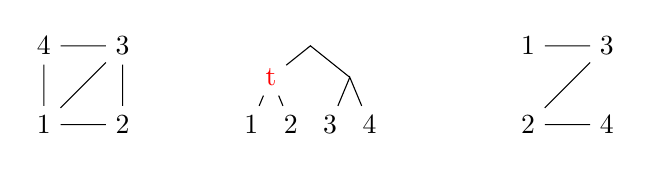
\begin{tikzpicture}
			\node (v1) at (0, 0){1};
			\node (v2) at (1, 0){2};
			\node (v3) at (1, 1){3};
			\node (v4) at (0, 1){4};
		
			\draw (v3) -- (v1) -- (v2) -- (v3) -- (v4) -- (v1);
		
		\begin{scope}[xshift = 75]
			\node (t1) at (0, 0){1};
			\node (t2) at (.5, 0){2};
			\node (t3) at (1, 0){3};
			\node (t4) at (1.5, 0){4};
			\node (t5) at (.25, .6){\color{red}t};
			\node (t6) at (1.25,.6){};
			\node (t7) at (.75, 1){};
			\draw (t1) -- (t5) -- (t2) (t3) -- (1.25, .6) -- (t4) (t5) to (.75, 1) to (1.25, .6);
		
		
		\end{scope}
		\begin{scope}[xshift = 175]
			\node (x1) at (0, 1){1};
			\node (x2) at (0, 0){2};
			\node (x3) at (1, 1){3};
			\node (x4) at (1, 0){4};
		
			\draw (x1) -- (x3) -- (x2) -- (x4);
		\end{scope}
		\end{tikzpicture}
	\end{center}}
	\uncover<5->{MIM-width($t$) = 2.}
\end{frame}
\begin{frame}[t]{Structuredness of a formula}
	\begin{itemize}[<+->]
		\item Let $\varphi$ be a DNNF formula and let $V := \mathrm{VAR}(\varphi)$.
		\item A \textbf{$\mathbf{v}$Tree} $T$ is a binary tree where the leaves of the tree has a one-to-one correspondence to the variables of $\varphi$.
		\item The formula $\varphi$ respects $T$ if and only if for each subformula of  $\varphi$ of the form $\varphi' := \psi_1 \land \psi_2$, there is a vertex $v \in V(T)$ with two children $v_1, v_2$, where $\mathrm{VAR}(\psi_1)\subseteq V(T_{v_1})$ and $\mathrm{VAR}(\psi_2) \subseteq V(T_{v_2})$, where $T_v$ is the subtree of $T$ rooted at $v$. We say $\varphi'$ respects $v$ in this case.
		\item A formula $\varphi$ is structured, if there is a $v$tree $T$ over the vertices of $\varphi$, such that $\varphi$ respects $T$.
	\end{itemize}

	\uncover<3->{
	\begin{minipage}{.49\linewidth}
		$$(x\land(y\lor z)) \lor (z \textcolor{red}{\bm{\land}} \lnot x)$$
	\end{minipage}
	\hfill
	\begin{minipage}{.49\linewidth}
		\centering
		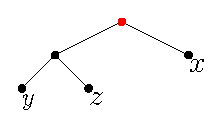
\includegraphics[width=.6\linewidth]{figures/vtree.eps}
	\end{minipage}
	}
\end{frame}

\begin{frame}[t]{Incidence graphs and structure of formulas}
	\begin{itemize}
		\item The \textbf{incidence graph} of $\mathcal{H}$ is a 
		\item[] \hspace{1cm}bipartite graph $(V(\mathcal{H}) \cup E(\mathcal{H}), E)$
		\item[] \hspace{1cm},where $\{v, e\} \in E$ iff $v \in e$.
			\vspace{.5cm}

		\uncover<2->{\item The incidence graph of a CNF-Formula is
		\item[] \hspace {1cm} the incidence graph of its hyper graph.}

			\vspace{.5cm}
		\uncover<3->{\item The MIM-width of a CNF-formula is the MIM-width of its incidence graph.}
	\end{itemize}

\end{frame}
\begin{frame}{Results on the structured d-DNNF}
\end{frame}
